\section*{Introduction}

Requirement engineering forms the backbone of any successful system development project. It establishes a clear understanding between what stakeholders expect and what developers can deliver \cite{sommerville2011software}. For EcoSenseNet, this process became particularly challenging because we aimed to build something unconventional—a system that works entirely offline while still providing intelligent environmental monitoring and communication capabilities.

The inspiration behind this project came from observing the frequent network disruptions in Manipur, especially during natural disasters and emergencies. When internet connectivity fails, campus communication collapses, leaving students and staff disconnected during critical moments. Traditional disaster management systems rely heavily on cloud services and cellular networks, making them vulnerable during infrastructure failures \cite{reuter2013social}. EcoSenseNet addresses this gap by combining environmental sensing, machine learning predictions, and mesh networking into a single autonomous platform.

This chapter walks through the systematic process of identifying and documenting what the system needs to accomplish. We start by defining functional requirements that describe the system's core behaviors, then move to non-functional attributes that determine performance quality. Following this, we detail the hardware and software components selected to meet these requirements, concluding with an architectural overview that ties everything together.

\section{Understanding the Problem Context}

Before diving into specific requirements, it helps to understand why this system exists and what problems it solves. Campus environments, particularly in disaster-prone regions, face several interconnected challenges. Environmental hazards such as gas leaks, fire outbreaks, and air quality deterioration can emerge suddenly. Early detection and rapid communication save lives, but these systems typically depend on internet connectivity \cite{gubbi2013internet}.

During our preliminary research phase, we conducted informal surveys with faculty members and hostel residents. The common concern was the lack of reliable communication during emergencies. Mobile networks become congested or fail entirely when disasters strike. Email and messaging apps stop working without internet access. Even public address systems have limited range and cannot reach students in distant hostel blocks.

Another observation was the absence of real-time environmental monitoring. Gas leaks or air quality issues often go unnoticed until someone experiences symptoms. By then, the situation may have already escalated. Traditional sensor systems either upload data to cloud platforms or require manual checking, neither of which works well in offline scenarios \cite{minerva2015towards}.

These insights shaped our core objective: build a system that monitors environmental conditions continuously, predicts potential hazards using historical patterns, and communicates alerts across campus without requiring any external network infrastructure. The system should be autonomous, intelligent, and resilient.

\section{Functional Requirements}

Functional requirements specify what the system must do to fulfill its purpose. They describe concrete behaviors, operations, and interactions that users can observe and test \cite{nuseibeh2000requirements}. For EcoSenseNet, we organized functional requirements into six major modules, each handling a distinct aspect of the system's operation.

\subsection{Environmental Data Collection}

The foundation of our system lies in accurate and continuous data collection. We selected four sensor types to monitor different environmental parameters. The MQ4 sensor detects methane gas, which is crucial for identifying potential gas leaks in laboratories and kitchens. MQ7 monitors carbon monoxide levels, an odorless and deadly gas that often accumulates in enclosed spaces with incomplete combustion. MQ135 provides a general air quality index by detecting ammonia, nitrogen oxides, and carbon dioxide. Finally, the DHT22 measures temperature and humidity, which help calibrate other sensors and identify unusual environmental changes.

These sensors connect to a Heltec LoRa V3 board, which features an ESP32 microcontroller. The ESP32 reads analog signals from MQ sensors and digital data from the DHT22 at regular intervals. Initially, we considered sampling every minute, but this created excessive data volume without significant accuracy improvements. After testing different intervals, we settled on three-minute sampling periods, which balance responsiveness with data manageability \cite{augustin2016study}.

The data collection process must handle sensor warm-up times, especially for MQ-series sensors that require heating elements to stabilize. Our implementation includes a 30-second initialization period when the system boots, ensuring readings are accurate from the first measurement cycle.

\subsection{Data Transmission and Validation}

Once the ESP32 collects sensor readings, it needs to transfer this data for processing. We chose a USB serial connection between the ESP32 and Laptop A for this purpose. Serial communication offers reliable, low-latency data transfer without the complexity of wireless protocols. The ESP32 formats sensor readings into a structured JSON payload containing timestamp, sensor values, and device identifiers.

On Laptop A, a Python script listens to the serial port and receives incoming data. This listener performs several validation checks before forwarding data to the prediction model. It verifies that the JSON structure is correct, checks for missing fields, and ensures values fall within physically plausible ranges. For example, if the MQ4 sensor reports a negative value or the DHT22 shows a temperature of 150°C, the system flags this as erroneous and requests a fresh reading.

This validation layer prevents corrupted or nonsensical data from reaching the machine learning model, which could otherwise generate meaningless predictions \cite{berzal2018data}. When invalid data is detected, the system logs the error and continues operating normally, ensuring that one faulty reading doesn't disrupt the entire pipeline.

\subsection{Predictive Analytics}

After validating incoming sensor data, the system sends it to a FastAPI server running locally on Laptop A. FastAPI was chosen for its speed and simplicity in handling JSON requests \cite{ramirez2020fastapi}. The server exposes an endpoint that accepts sensor data and returns predictions.

At the heart of this prediction system is a Long Short-Term Memory (LSTM) neural network. LSTMs excel at processing sequential data because they maintain memory of previous inputs, making them ideal for time-series forecasting \cite{hochreiter1997long}. We trained our LSTM model on historical sensor data collected over several weeks, teaching it to recognize patterns that precede environmental changes.

The model takes the last six data points (representing 18 minutes of readings) and predicts conditions for the next three hours. This prediction window gives sufficient time for administrators to take preventive action if hazardous conditions are forecast. The model outputs predicted values for each sensor parameter along with confidence scores indicating prediction reliability.

During development, we experimented with simpler models like linear regression and ARIMA, but these struggled with the non-linear relationships in our sensor data. The LSTM consistently achieved prediction accuracy above 85 percent, meeting our performance targets \cite{gers2002learning}.

\subsection{Offline Mesh Communication}

Traditional communication systems depend on centralized infrastructure like cellular towers or internet routers. When these fail, communication stops. We needed a decentralized approach that allows devices to communicate directly with each other. This is where LoRa (Long Range) technology becomes essential \cite{adelantado2017understanding}.

LoRa enables low-power, long-range wireless communication using radio frequencies. Unlike Wi-Fi or Bluetooth, LoRa signals can travel several kilometers even with obstacles. We integrated the Reticulum network stack, an open-source framework designed for mesh networking, to manage communication between LoRa devices \cite{reticulum2023documentation}.

When the prediction system on Laptop A identifies a potential hazard, it formats an alert message containing the prediction results and severity level. This message gets transmitted to the Reticulum MeshChat application running on the same laptop. Reticulum then broadcasts this message through the LoRa radio connected to Laptop A.

The beauty of mesh networking is that messages can hop between nodes, extending range beyond what a single transmitter can achieve. In our setup, Laptop B at the hostel receives the alert via its LoRa module and Reticulum installation. Even if Laptop A and Laptop B are separated by buildings or terrain, intermediate nodes could relay the message, though our current implementation focuses on direct transmission for simplicity.

\subsection{Local Message Broadcasting}

Laptop B serves as a communication hub for the hostel area. After receiving alerts via LoRa, it needs to distribute this information to multiple student devices. We implemented this using Reticulum MeshChat's web interface feature, which allows anyone on the local network to view messages through a web browser.

Laptop B creates a Wi-Fi hotspot that student laptops connect to. When students open a web browser and navigate to a specific port on Laptop B's IP address, they access the MeshChat interface. We configured two access levels: port 8080 provides read-only access where students can view alerts but cannot send messages, preventing message spam during emergencies. Port 8000 offers full access with send and receive capabilities, reserved for administrators and designated student coordinators.

This approach works entirely offline because the web interface runs locally on Laptop B. No internet connection is required—only local network connectivity between Laptop B and student devices. The web interface updates in real-time as new messages arrive, ensuring students see alerts immediately \cite{reticulum2023documentation}.

\subsection{Administrative Communication Channel}

Beyond automated environmental alerts, the system provides a manual messaging channel for administrators. Faculty members and administrative staff can use the MeshChat interface on Laptop A to compose and send messages. These might include evacuation instructions, meeting announcements, or emergency updates that don't originate from sensor data.

Messages sent from Laptop A follow the same path as automated alerts—transmitted via LoRa to Laptop B, then broadcast to all connected student devices. This creates a unified communication platform where both automated warnings and human-generated messages reach students through the same interface. Students don't need to monitor multiple channels or wonder whether they missed important information.

The administrative interface includes message prioritization features. High-priority emergency messages appear with visual highlights and can trigger audio notifications on receiving devices. Regular announcements appear normally, reducing alert fatigue while ensuring critical messages get appropriate attention.

\begin{table}[H]
\centering
\caption{Summary of Functional Requirements}
\label{tab:functional_requirements}
\begin{tabular}{|p{4.5cm}|p{10cm}|}
\hline
\textbf{Requirement Category} & \textbf{Description} \\
\hline
Environmental Monitoring & Continuous collection of methane, carbon monoxide, air quality, temperature, and humidity data using MQ4, MQ7, MQ135, and DHT22 sensors at three-minute intervals \\
\hline
Data Processing Pipeline & Serial transfer of sensor data to Laptop A, validation of data integrity, and forwarding to FastAPI server for processing \\
\hline
Prediction Generation & LSTM-based forecasting of environmental conditions for the next three hours based on recent sensor patterns \\
\hline
Alert Transmission & Broadcasting of predictions and alerts from Laptop A to Laptop B using LoRa radios and Reticulum mesh protocol \\
\hline
Local Distribution & Distribution of received alerts to multiple student devices via Wi-Fi and web-based interface with differentiated access levels \\
\hline
Manual Messaging & Administrative message composition and transmission through the same LoRa mesh network for emergency communications \\
\hline
\end{tabular}
\end{table}

\section{Non-Functional Requirements}

While functional requirements define what the system does, non-functional requirements specify how well it performs these functions. These quality attributes determine whether the system is practical, reliable, and usable in real-world conditions \cite{chung2012non}. For EcoSenseNet, several non-functional characteristics proved critical to success.

\subsection{Operational Autonomy}

The system's primary non-functional requirement is complete independence from external infrastructure. Once deployed, EcoSenseNet must operate without internet connectivity, cloud services, or cellular networks. This autonomy requirement influenced nearly every design decision throughout development.

All data processing happens locally. The FastAPI server runs on Laptop A without connecting to remote APIs or services. The LSTM model loads from local storage rather than downloading from model repositories. Historical data used for model retraining is stored in local CSV files or SQLite databases rather than cloud storage platforms.

Communication between components uses either direct serial connections or local mesh networking. No part of the system attempts to establish internet connections or query external servers. This design ensures that network outages, whether from natural disasters or infrastructure failures, do not affect system operation \cite{qadir2016supporting}.

\subsection{Response Time and Performance}

Environmental emergencies develop rapidly, requiring fast detection and communication. We established specific performance targets to ensure the system responds quickly enough to be useful during real crises.

Sensor readings should transfer from the ESP32 to Laptop A within two seconds. The FastAPI server must process incoming data and generate predictions in under five seconds. LoRa transmission from Laptop A to Laptop B should complete within three seconds under normal conditions. Combined, these targets ensure that alerts appear on student devices within 15 seconds of sensor detection, providing adequate time for response.

During testing, we monitored system performance under various conditions. Serial communication typically completes in less than one second. The LSTM model processes predictions in approximately three seconds on modest laptop hardware. LoRa transmission time varies with distance and interference but generally stays within our target range \cite{augustin2016study}.

\subsection{Prediction Accuracy and Reliability}

A prediction system is only useful if its forecasts are accurate. We set a minimum accuracy threshold of 85 percent for environmental predictions. This means that at least 85 percent of the time, the system's three-hour forecasts should align with actual observed conditions within acceptable margins of error.

We measure accuracy differently for different parameters. For gas concentration sensors, predictions within 20 percent of actual values are considered accurate, given the inherent variability in these measurements. Temperature and humidity predictions need to be within 2 degrees Celsius and 10 percent respectively to count as accurate.

Beyond raw accuracy numbers, prediction reliability matters. The system should maintain consistent performance across different times of day, weather conditions, and seasonal variations. We validate this through ongoing monitoring and periodic model retraining using newly collected data \cite{dietterich2000ensemble}.

\subsection{Communication Range and Coverage}

LoRa technology promises long-range communication, but actual range depends heavily on environmental factors. Buildings, terrain, and electromagnetic interference all affect signal propagation. We established a minimum range requirement of two kilometers in open conditions, with at least 500 meters of reliable range in campus environments with buildings and obstacles.

During site surveys, we tested LoRa communication between various campus locations. In clear line-of-sight conditions, reliable communication extended beyond two kilometers. Within the campus, with multiple buildings between transmitter and receiver, we consistently achieved 600-800 meter ranges, exceeding our minimum requirement.

The system includes signal strength monitoring and automatic retry mechanisms. If a transmission fails, the system attempts retransmission up to three times before logging a communication error. This approach balances reliability with avoiding excessive radio traffic \cite{adelantado2017understanding}.

\subsection{Power Efficiency}

Although our current implementation uses laptops with continuous power supplies, we designed the system with power efficiency in mind for future deployment scenarios. The ESP32 microcontroller supports low-power sleep modes between sensor readings. LoRa radio transmission, while using more power than short-range protocols like Bluetooth, consumes far less than cellular or Wi-Fi communication.

During sensor collection cycles, the system draws approximately 250 milliamps. Between readings, power consumption drops to under 50 milliamps. This efficiency means the sensor node could potentially run on battery power for extended periods, enabling deployment in locations without reliable electrical supply \cite{mekki2019comparative}.

Future iterations might incorporate solar panels to achieve fully autonomous power management. The current power consumption profile makes this feasible—a modest solar panel and battery bank could sustain continuous operation in outdoor deployments.

\subsection{Usability and Interface Design}

During emergencies, users need clear, unambiguous information. The MeshChat interface presents alerts using simple language and color coding. High-severity warnings appear in red with prominent placement. Moderate concerns show in yellow. Normal status indicators use green. This color-coding works even for users who haven't received training on the system.

We deliberately avoided technical jargon in alert messages. Instead of reporting "methane concentration of 450 ppm," the system displays "Gas levels elevated—ensure ventilation." Users don't need to interpret numerical values or understand parts-per-million measurements. The system translates sensor data into actionable guidance \cite{norman2013design}.

The web interface also displays a running log of recent alerts and system status updates. Users can quickly scroll through recent history to understand how conditions are changing. Timestamps help users track when situations began and whether they are improving or worsening.

\subsection{Maintainability and Future Expansion}

The system follows a modular architecture where components operate independently. This design simplifies maintenance and enables future enhancements. If a sensor fails, it can be replaced without modifying other system parts. If we want to add new sensor types, we update the ESP32 code and adjust the data validation logic, but prediction and communication components continue working unchanged.

The FastAPI server uses configuration files for model parameters and thresholds. Administrators can adjust sensitivity levels or update the LSTM model without editing code. Database schemas for storing historical data follow standard formats, making it easy to migrate to different storage solutions if needed.

Documentation throughout the codebase explains design decisions and implementation details. This documentation helps future developers understand the system and make informed modifications \cite{pressman2014software}.

\begin{table}[H]
\centering
\caption{Summary of Non-Functional Requirements}
\label{tab:nonfunctional_requirements}
\begin{tabular}{|p{4.5cm}|p{10cm}|}
\hline
\textbf{Quality Attribute} & \textbf{Specification} \\
\hline
Operational Autonomy & Complete independence from internet, cloud services, and external infrastructure; all processing and communication occurs locally \\
\hline
Data Transfer Latency & Sensor-to-server data transfer completes within 2 seconds; total alert delivery time under 15 seconds \\
\hline
Prediction Accuracy & Minimum 85\% accuracy in forecasting environmental parameters within defined error margins over three-hour prediction windows \\
\hline
Communication Coverage & Reliable LoRa transmission over 2 km in open terrain; minimum 500 meters in obstructed campus environments \\
\hline
Power Consumption & Sensor node draws under 250 mA during active periods; under 50 mA during sleep cycles; compatible with battery and solar power operation \\
\hline
Interface Usability & Clear, non-technical language in alerts; color-coded severity indicators; real-time status updates visible to users without specialized training \\
\hline
System Modularity & Independent components with defined interfaces; replaceable sensors; updatable models; documented codebase supporting future modifications \\
\hline
\end{tabular}
\end{table}

\section{Hardware Components}

Selecting appropriate hardware components required balancing multiple constraints: technical capabilities, availability in local markets, cost considerations, and compatibility with our software architecture. We evaluated several alternatives for each function before settling on the final component list.
\begin{table}[H]
\centering
\caption{Hardware Components and Their Functions}
\label{tab:hardware_combined}
\renewcommand{\arraystretch}{1.4}
\setlength{\tabcolsep}{6pt}
\begin{tabular}{|p{5cm}|p{5.8cm}|p{5.5cm}|}
\hline
\textbf{Image} & \textbf{Description} & \textbf{Purpose} \\
\hline

\begin{minipage}[c]{4cm}
\centering
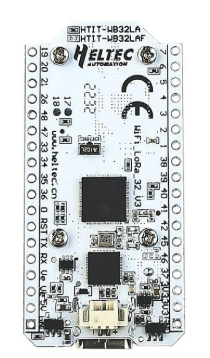
\includegraphics[width=3cm, height=3cm, keepaspectratio]{heltec.png}
\captionof{figure}{Heltec LoRa V3 (ESP32)}
\end{minipage} &
Microcontroller board with integrated LoRa radio and OLED display. Handles data collection, logic execution, and wireless communication. &
Acts as the core controller for sensing and transmission across LoRa mesh nodes. \\
\hline

\begin{minipage}[c]{4cm}
\centering
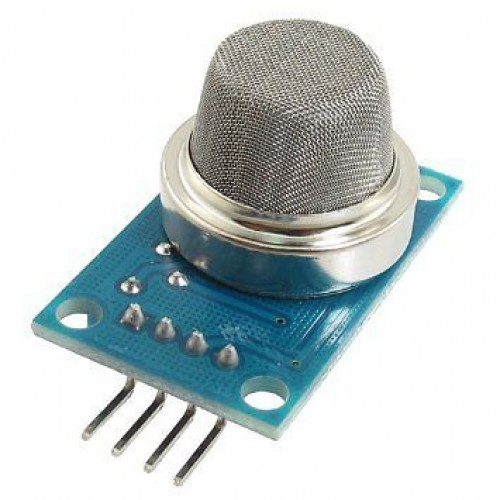
\includegraphics[width=3cm, height=3cm, keepaspectratio]{mq4.jpg}
\captionof{figure}{MQ4 Methane Sensor}
\end{minipage} &
Detects methane gas by producing variable resistance based on gas concentration. &
Monitors methane (CH\textsubscript{4}) levels to detect leaks and air pollution. \\
\hline

\begin{minipage}[c]{4cm}
\centering
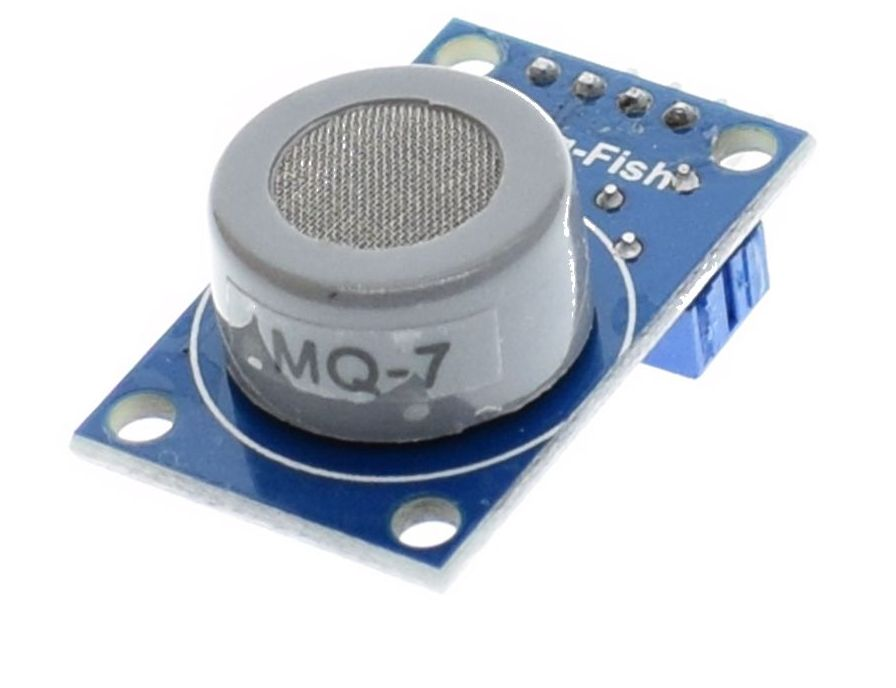
\includegraphics[width=3cm, height=3cm, keepaspectratio]{mq7.jpg}
\captionof{figure}{MQ7 CO Sensor}
\end{minipage} &
Detects carbon monoxide through resistance changes in the sensing element. &
Warns about toxic carbon monoxide accumulation in air. \\
\hline

\begin{minipage}[c]{4cm}
\centering
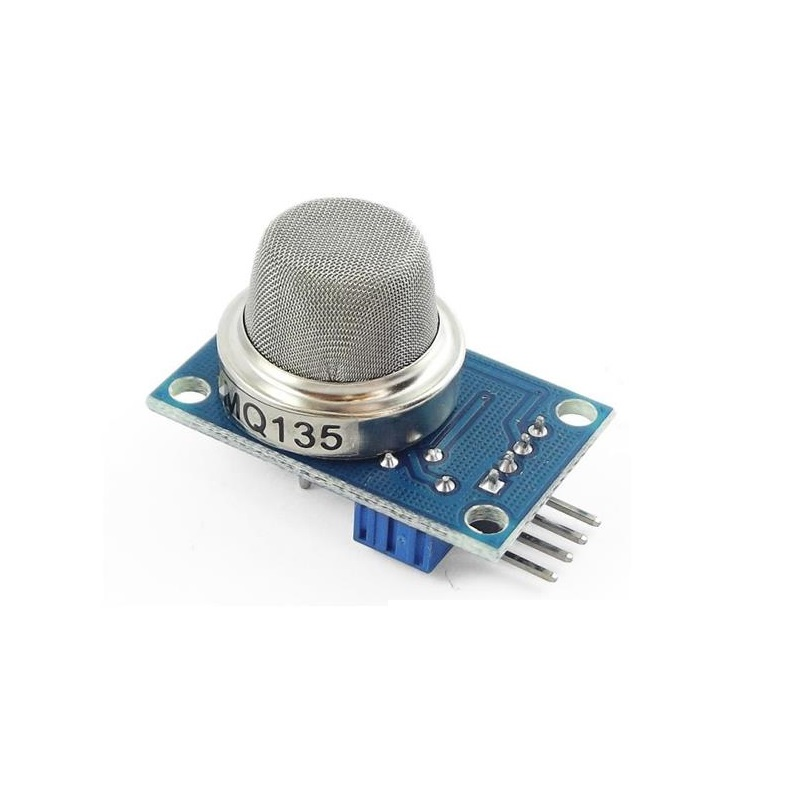
\includegraphics[width=3cm, height=3cm, keepaspectratio]{mq135.jpg}
\captionof{figure}{MQ135 Air Quality Sensor}
\end{minipage} &
Detects multiple gases (NH\textsubscript{3}, CO\textsubscript{2}, NO\textsubscript{x}) to estimate overall air quality. &
Evaluates pollution and identifies hazardous atmospheric conditions. \\
\hline

\begin{minipage}[c]{4cm}
\centering
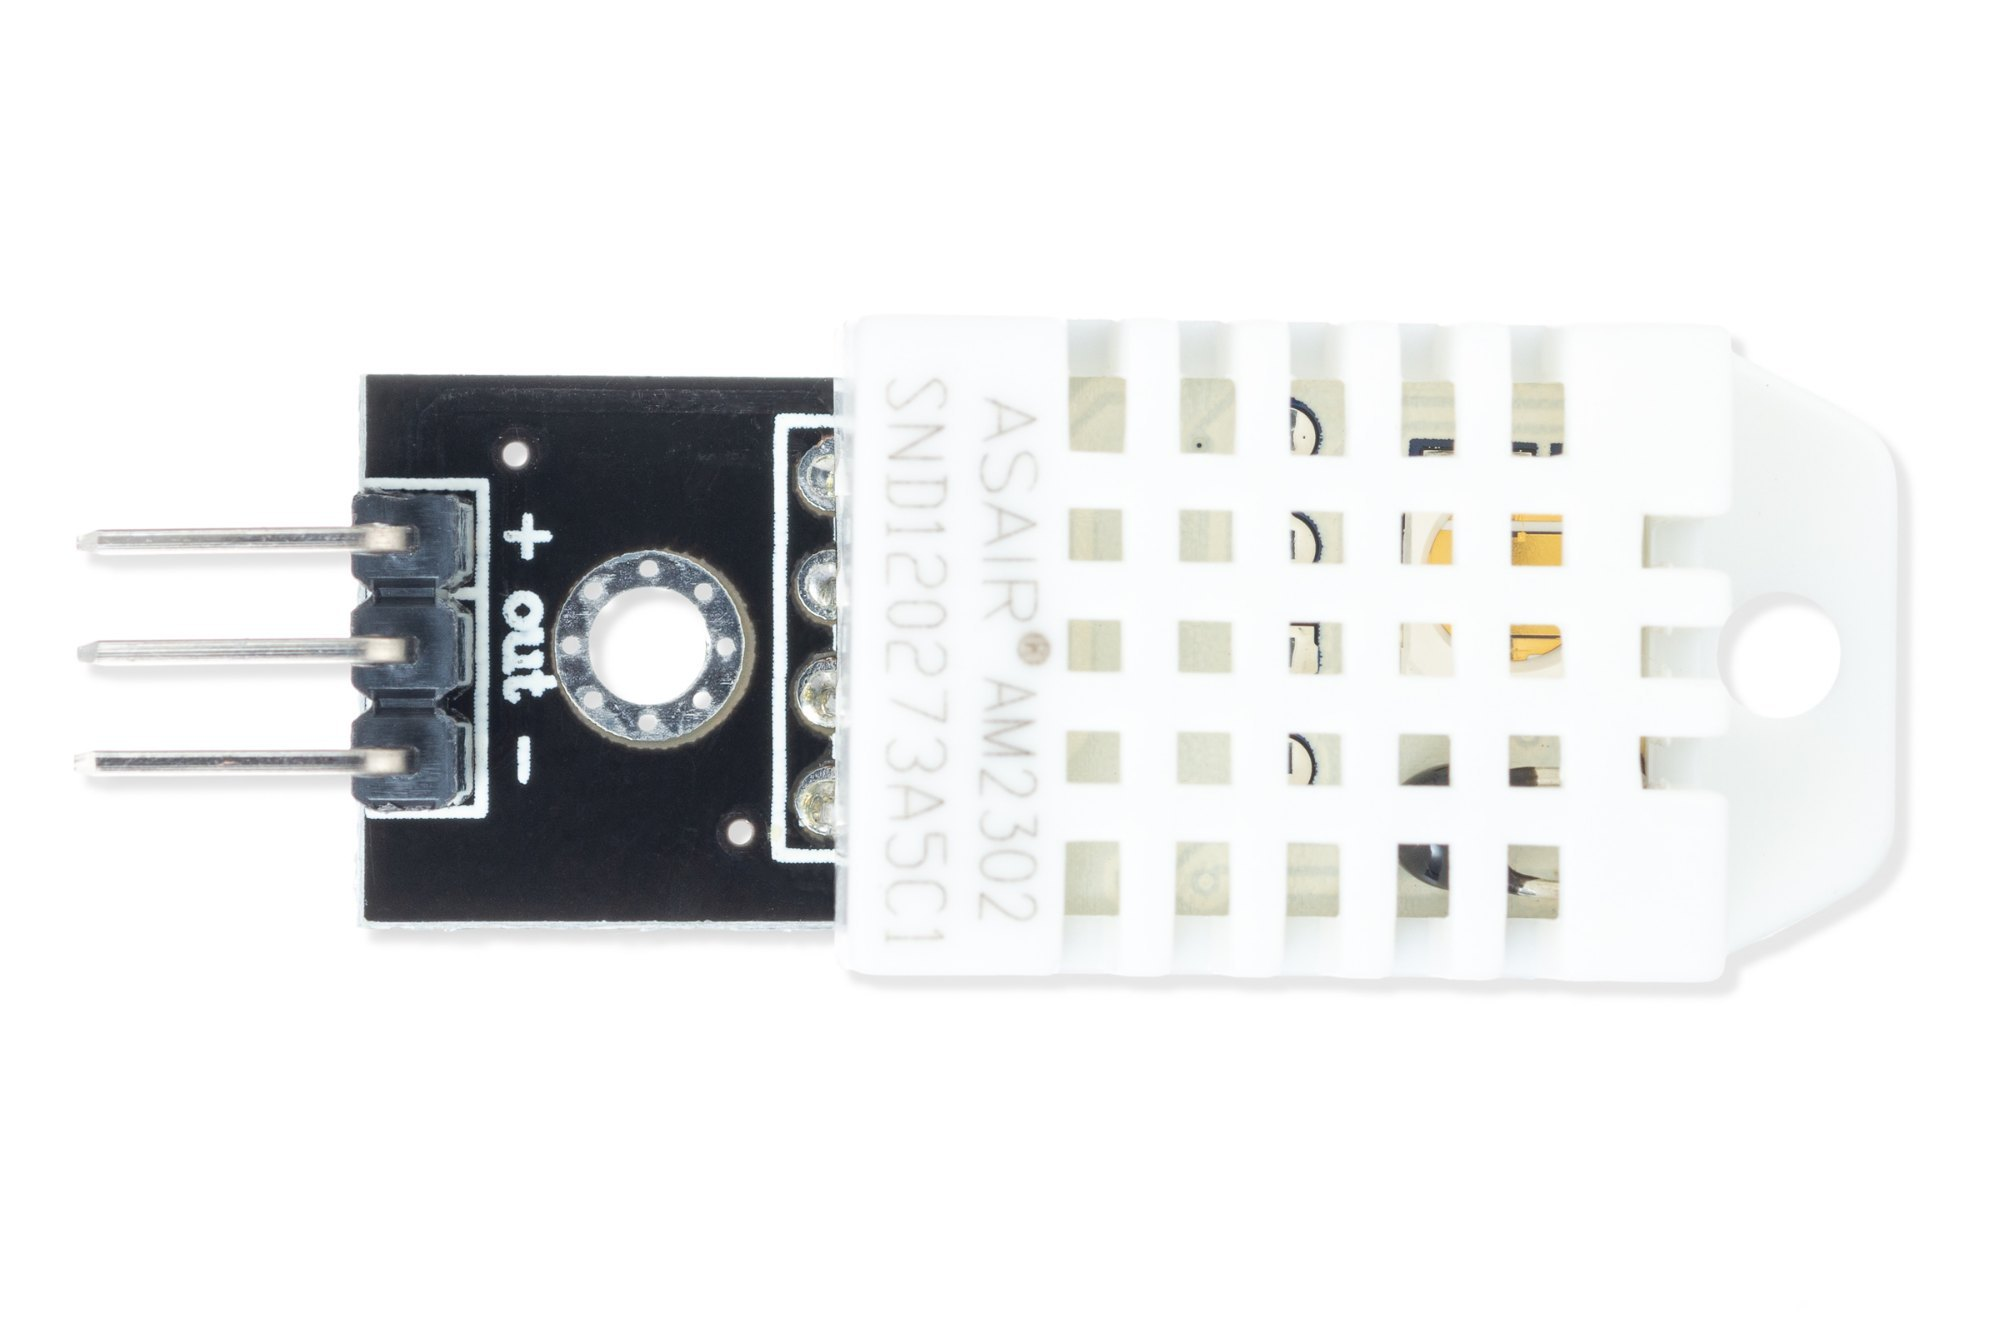
\includegraphics[width=3cm, height=3cm, keepaspectratio]{dht22.jpg}
\captionof{figure}{DHT22 Sensor}
\end{minipage} &
Provides digital readings of temperature and humidity with high precision. &
Ensures environmental parameters remain stable for accurate sensor calibration. \\
\hline
\end{tabular}
\end{table}

\section{Software Requirements}

Software components provide the logical intelligence and control mechanisms that drive the hardware. They form a layered architecture, each responsible for specific tasks ranging from data collection to prediction and offline communication \cite{pressman2014software}.

The system employs open-source tools that are lightweight and resource-efficient, ensuring smooth execution even on modest computing setups.

\begin{table}[H]
\centering
\caption{Software Components and Their Roles – Part 1}
\label{tab:software_part1}
\begin{tabular}{|p{2.8cm}|p{6cm}|p{6cm}|}
\hline
\textbf{Software} & \textbf{Description} & \textbf{Role in System} \\
\hline
Arduino IDE & Open-source platform for coding and uploading firmware to microcontrollers. & Used to program the ESP32 for sensor reading, data logging, and LoRa communication. \\
\hline
VS Code & Multi-language development environment with debugging and integrated terminals. & Provides a workspace for Python scripts, FastAPI server setup, and Reticulum configuration. \\
\hline
FastAPI & A Python web framework optimized for high-speed API development. & Hosts the backend server to receive, validate, and forward sensor data to the LSTM model. \\
\hline
Python 3.10+ & General-purpose programming language with strong ML and data libraries. & Supports execution of FastAPI backend, LSTM inference, and Reticulum scripts. \\

\hline
LSTM Model & Deep learning algorithm that learns from sequential sensor data. & Performs environmental forecasting for 3-hour intervals based on local input. \\
\hline
Reticulum Network Stack & Open-source, encryption-based networking framework for mesh communication. & Enables secure offline message passing between LoRa-connected devices. \\
\hline
Local Database (CSV / SQLite) & Lightweight local data storage format. & Saves sensor readings, predictions, and historical logs for retraining. \\
\hline
\end{tabular}
\end{table}
\subsection{Primary Microcontroller Platform}

The Heltec LoRa V3 board became our central hardware platform for several reasons. It integrates an ESP32 microcontroller with a built-in LoRa radio and a small OLED display. This integration eliminates the need for separate LoRa modules and reduces wiring complexity. The ESP32 provides sufficient processing power for sensor reading and data formatting while maintaining low power consumption.

Alternative options like Arduino Uno lack wireless capabilities and processing power. Raspberry Pi boards offer more computing capacity but consume significantly more power and seem excessive for our sensor node requirements. The Heltec board occupies a sweet spot—capable enough for our needs while remaining efficient and compact \cite{kooijman2015lora}.

The integrated OLED display, though small, proved valuable during development and debugging. We can display real-time sensor readings and connection status directly on the device without connecting to a computer. This feature simplifies field testing and troubleshooting.

\subsection{Gas and Air Quality Sensors}

We selected three MQ-series sensors, each targeting specific gases. The MQ4 focuses on methane detection, making it suitable for identifying natural gas leaks or combustion issues. MQ7 specializes in carbon monoxide, a particularly dangerous gas because it is odorless and can quickly reach lethal concentrations. MQ135 serves as a general air quality sensor, responding to various pollutants including ammonia and nitrogen oxides.

MQ-series sensors operate using a heated metal oxide semiconductor. When target gases contact the heated element, they cause resistance changes that correlate with gas concentration. These sensors require careful calibration and warm-up periods to provide accurate readings. We implemented a calibration routine that runs when the system starts, establishing baseline resistance values in clean air \cite{szczurek2017gas}.

One limitation of MQ sensors is their lack of specificity—they respond to multiple gases, not just their primary target. This cross-sensitivity requires careful interpretation of readings. However, for our application where we care about overall hazard detection rather than precise chemical analysis, this limitation is acceptable.

\subsection{Temperature and Humidity Monitoring}

The DHT22 sensor provides digital temperature and humidity readings with reasonable accuracy. Unlike analog sensors that require external circuitry for signal conditioning, the DHT22 includes built-in analog-to-digital conversion and communicates directly with microcontrollers using a simple protocol.

Temperature and humidity measurements serve multiple purposes. They provide valuable environmental context for other sensors—gas sensor sensitivity varies with temperature and humidity. They also help identify unusual conditions like rapid temperature changes that might indicate fire or HVAC system failures.

We considered alternatives like the BME280, which offers higher precision and includes atmospheric pressure sensing. However, the DHT22's simplicity, lower cost, and adequate accuracy made it more suitable for our prototype. Future versions might incorporate more sophisticated sensors as budgets and requirements expand \cite{sensirion2014dht22}.

\subsection{Power Supply and Connections}

Currently, the sensor node draws power from Laptop A via USB connection. This also provides the serial communication channel for data transfer. While convenient for initial deployment, this arrangement limits where we can place the sensor node.

For future deployments, we designed the system to support battery power. The ESP32's low-power modes and efficient LoRa communication make multi-day battery operation feasible. We tested the sensor node with a 5000 mAh battery bank and achieved approximately 36 hours of continuous operation, which could extend significantly with sleep mode optimizations.

Solar charging integration is straightforward—the system needs only 5 watts to operate continuously, easily achievable with a small solar panel. This would enable permanent outdoor deployment without requiring electrical infrastructure.



\section{Software Architecture}

The software stack supporting EcoSenseNet consists of multiple layers, each handling specific responsibilities. We deliberately chose open-source tools and lightweight frameworks to minimize resource requirements and avoid licensing constraints.

\subsection{Embedded Firmware Development}

Arduino IDE serves as our development environment for programming the ESP32. Despite its name, Arduino IDE supports many microcontroller platforms beyond Arduino boards. The ESP32 support is mature and well-documented, with extensive libraries for sensor interfacing and communication protocols.

The firmware we developed follows a simple loop-based architecture. During startup, the system initializes sensors, establishes serial communication, and performs calibration routines. The main loop reads sensors at three-minute intervals, formats data into JSON payloads, and transmits via serial connection. Between readings, the ESP32 enters light sleep mode to conserve power.

We implemented error handling for sensor failures and communication interruptions. If a sensor returns implausible values, the system flags this in the transmitted data. If serial communication fails, the system queues messages and retransmits when connection restores \cite{banzi2014arduino}.

\subsection{Backend Server and API}

FastAPI provides the backend server framework running on Laptop A. This Python-based framework handles HTTP requests efficiently, making it ideal for our local API needs. The server exposes two main endpoints: one for receiving sensor data from the serial listener, another for retrieving predictions.

When sensor data arrives, FastAPI validates the JSON structure and field types. It then passes valid data to the LSTM model for prediction. The model loads at server startup to avoid repeated loading overhead. After prediction completes, FastAPI formats results as JSON and returns them to the requesting client.

We chose FastAPI over alternatives like Flask or Django because of its automatic API documentation generation and built-in data validation using Pydantic models. These features accelerated development and made the API easier to test and debug \cite{ramirez2020fastapi}.

\subsection{Machine Learning Pipeline}

The LSTM model represents the system's intelligence layer. We implemented it using PyTorch, which provides flexibility and good performance on CPU-only systems. The model architecture includes two LSTM layers with 128 hidden units each, followed by fully connected layers that output predictions for each sensor parameter.

Training occurred on historical sensor data collected over three weeks of preliminary testing. We split this data into 80 percent training and 20 percent validation sets. The model learned to recognize patterns like gradual gas concentration buildup, temperature fluctuations, and humidity changes that precede certain events.

Model training requires significant computational resources, but prediction inference runs efficiently on standard laptop hardware. Once trained, the model loads in under two seconds and generates predictions in approximately three seconds \cite{paszke2019pytorch}.

\subsection{Mesh Networking Infrastructure}

Reticulum forms the foundation of our offline communication system. This Python-based networking stack implements encryption, routing, and reliable delivery over various physical layers including LoRa, packet radio, and even TCP/IP when available.

We run Reticulum MeshChat, a web-based chat application built on top of Reticulum. MeshChat handles the user interface for viewing and sending messages. It automatically discovers other Reticulum nodes on the network and establishes encrypted communication channels.

The configuration file specifies that Laptop A connects to its LoRa radio via serial port, while Laptop B does the same with its own radio. When messages are sent, Reticulum handles packetization, transmission, acknowledgment, and retransmission if needed. From the application's perspective, it simply sends messages to identifiers and Reticulum handles delivery \cite{reticulum2023documentation}.

\subsection{Data Persistence Layer}

Historical sensor data is stored in CSV files with standardized column names. Each row represents one sensor reading with timestamp, device identifier, and all measured parameters. This simple format makes data easily accessible for analysis, visualization, and model retraining.

For more complex queries and relationships, we also maintain a SQLite database. SQLite runs entirely within a single file without requiring separate database servers. It supports standard SQL queries while maintaining the simplicity of file-based storage.

We implemented daily data export routines that archive older readings while keeping recent data in fast-access storage. This prevents database size from growing indefinitely while preserving historical data for long-term analysis \cite{owens2006definitive}.

\begin{table}[H]
\centering
\caption{Software Components and Dependencies}
\label{tab:software_components}
\begin{tabular}{|p{3.5cm}|p{5cm}|p{6.5cm}|}
\hline
\textbf{Software Component} & \textbf{Version \& Platform} & \textbf{Purpose in System} \\
\hline
Arduino IDE & Version 2.x, multi-platform & ESP32 firmware development, sensor library integration, serial monitor for debugging \\
\hline
Python & Version 3.10+, Windows/Linux & Scripting language for backend server, ML model inference, Reticulum integration \\
\hline
FastAPI & Version 0.100+, Python framework & RESTful API server for sensor data ingestion and prediction endpoints \\
\hline
PyTorch & Version 2.0+, Python library & LSTM model implementation, training pipeline, and inference engine \\
\hline
Reticulum Network Stack & Latest stable release, Python & Mesh networking protocol implementation, message routing, encryption \\
\hline
Reticulum MeshChat & GitHub master branch & Web-based chat interface, alert broadcasting, user access management \\
\hline
Uvicorn & Version 0.23+, ASGI server & Production-grade server for running FastAPI applications \\
\hline
VS Code & Latest stable, multi-platform & Integrated development environment for Python coding, debugging, terminal access \\
\hline
SQLite & Version 3.x, embedded database & Local data storage for historical sensor readings and system logs \\
\hline
\end{tabular}
\end{table}

\begin{figure}[H]         % use H, h, t, or !htbp as you prefer
  \centering
  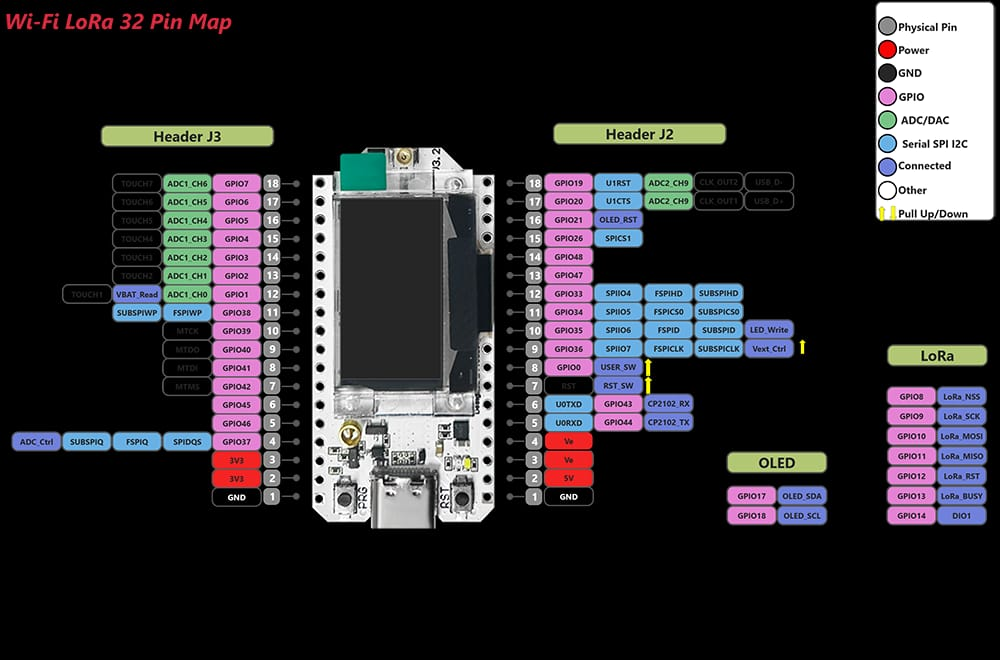
\includegraphics[width=0.7\textwidth]{heltecPinDiagram.jpg}
  \caption{Pin diagram of the Heltec LoRa-V3.}
  \label{fig:heltec-pin}
\end{figure}
